%%%%%%%%%%%%%%%%%%%%%%%%%%%%%%%%%%%%%%%%%
% University/School Laboratory Report
% LaTeX Template
% Version 3.1 (25/3/14)
%
% This template has been downloaded from:
% http://www.LaTeXTemplates.com
%
% Original author:
% Linux and Unix Users Group at Virginia Tech Wiki 
% (https://vtluug.org/wiki/Example_LaTeX_chem_lab_report)
%
% License:
% CC BY-NC-SA 3.0 (http://creativecommons.org/licenses/by-nc-sa/3.0/)
%
%%%%%%%%%%%%%%%%%%%%%%%%%%%%%%%%%%%%%%%%%

%----------------------------------------------------------------------------------------
%	PACKAGES AND DOCUMENT CONFIGURATIONS
%----------------------------------------------------------------------------------------

\documentclass{article}

\usepackage[version=3]{mhchem} % Package for chemical equation typesetting
\usepackage{siunitx} % Provides the \SI{}{} and \si{} command for typesetting SI units
\usepackage{graphicx} % Required for the inclusion of images
\usepackage{natbib} % Required to change bibliography style to APA
\usepackage{amsmath} % Required for some math elements 

\setlength\parindent{0pt} % Removes all indentation from paragraphs

\renewcommand{\labelenumi}{\alph{enumi}.} % Make numbering in the enumerate environment by letter rather than number (e.g. section 6)

%\usepackage{times} % Uncomment to use the Times New Roman font

%----------------------------------------------------------------------------------------
%	DOCUMENT INFORMATION
%----------------------------------------------------------------------------------------

\title{Circular Motion and Gravity \\ Orbital Simulation \\ PHYS 442} % Title

\author{Dr. Schultz } % Author name

\date{\today} % Date for the report

\begin{document}

\maketitle % Insert the title, author and date

\begin{center}
\begin{tabular}{l r}
Date Performed: & September 18, 2015 \\ % Date the experiment was performed
Partners: & Whole class \\ % Partner names
Instructor: & Me % Instructor/supervisor
\end{tabular}
\end{center}

% If you wish to include an abstract, uncomment the lines below
% \begin{abstract}
% Abstract text
% \end{abstract}

%----------------------------------------------------------------------------------------
%	SECTION 1
%----------------------------------------------------------------------------------------

\section{Objective}

Explored the motion of a particle under the influence of a gravitational force. Specifically we look at attractive inverse square distance forces, Hookean forces, escape velocity, circular orbits, kinetic energy, potential energy and elliptical orbits.  These are defined in \ref{definitions}:


% If you have more than one objective, uncomment the below:
%\begin{description}
%\item[First Objective] \hfill \\
%Objective 1 text
%\item[Second Objective] \hfill \\
%Objective 2 text
%\end{description}

\subsection{Definitions}
\label{definitions}
\begin{description}
\item[Law of Universal Gravitation]
The law of universal gravitation states the force of gravity between two point masses is directly proportional to each mass and inversely proportional to the distance between them.  This is also true for masses outside of spherically symmetric mass distributions.\cite{Homer:2014}
$$ F_g=\frac{mMG}{r^2}$$
\item[Hookean Forces]
Inside a uniformly dense sphere of mass the force is Hookean, with an attractive force proportional to the displacement from equilibrium.  The effective spring constant is $K=\frac{mMG}{R^3}$.
$$ F_g=\frac{mMG}{R^3}r$$
\item[Gravitational Constant]
The universal gravitation constant G determines the strength of the gravity force from a given mass.  It may also be considered as the force that 1 kg exerts on another 1 kg mass separated by 1 meter.\\
$$G=6.67\times 10^{-11}\frac{Nm^2}{kg^2}$$
\item[Escape Velocity]
Escape velocity is the initial velocity required to escape gravitational attraction.  An object launched at the escape velocity will never come back (escape).\\
$$v_{escape}=\sqrt{\frac{2MG}{r}}$$
\item[Kinetic Energy]
Kinetic energy is the energy associated with motion.  \\
$$KE=\frac{mv^2}{2}$$
\item[Potential Energy]
The potential associated with the universal gravitation force is written as follows.  \\
$$PE=-\frac{mMG}{r}$$
\item[Circular Orbit]
A circular orbit is an orbit with a constant radius r.
\item[Elliptic Orbit]
An elliptic orbit is a closed orbit with changing radius r.
\end{description} 
 
%----------------------------------------------------------------------------------------
%	SECTION 2
%----------------------------------------------------------------------------------------

\section{Simulation}

The simulation applies a central acceleration to the orbiting particle.  Outside the boundary of the central mass we have the following acceleration.

$$a=\frac{K}{r^2}$$

Inside the boundary of the central mass ($r<R$) we have the following acceleration.

$$a=\frac{K}{R^3}r$$

Here R is the radius of the central mass and K is a constant determined by the user of the simulation.  K is MG.  For this simulation the radius was set to $R=6$ and the constant was set to $K=-0.1$ making the acceleration attractive.\\

The initial position $\overrightarrow{r}_0$ and initial velocity $\overrightarrow{v}_0$ are set by the user.

\newpage
%----------------------------------------------------------------------------------------
%	SECTION 3
%----------------------------------------------------------------------------------------

\section{Sample Calculation}
\subsection{Circular Orbit}
Given $\overrightarrow{r}_0=(10,0)$ and $K=-0.1$ we find the $\overrightarrow{v}_0$ for circular orbit.
$$F_{net}=ma$$
$$ \frac{mMG}{r^2} = m \frac{v^2}{r}$$
$$ \frac{K}{r^2} = \frac{v^2}{r}$$
$$v=\sqrt{\frac{K}{r}}$$
$$v=\sqrt{\frac{0.1}{10}}=0.1$$
The velocity must be tangential and therefore $\overrightarrow{v}_0$ must be perpendicular to $\overrightarrow{r}_0$.
$$\overrightarrow{v}_0=(0,0.1)$$

\subsection{Escape Velocity}
Given $\overrightarrow{r}_0=(10,0)$ and $K=-0.1$ we find the $\overrightarrow{v}_0$ for escape from the central mass' gravitational attraction.  Escape is associated with a total mechanical energy of zero.

$$PE+KE=0$$
$$-\frac{mMG}{r}+\frac{mv^2}{2}=0 $$
$$-\frac{K}{r}+\frac{v^2}{2}=0 $$
$$v_{escape}=\sqrt{\frac{2K}{r}}$$
$$v_{escape}=\sqrt{\frac{2(0.1)}{10}}=0.14$$

%----------------------------------------------------------------------------------------
%	SECTION 4
%----------------------------------------------------------------------------------------
\newpage 

\section{Results and Conclusions}

\subsection{Circular Orbit}
For the conditions $\overrightarrow{r}_0=(10,0)$ and $K=-0.1$ we calculate an initial velocity $\overrightarrow{v}_0=(0,0.1)$ will give a circular orbit.  Running the simulation yields the following orbit.  We can see it is circular.

\begin{figure}[h]
\begin{center}
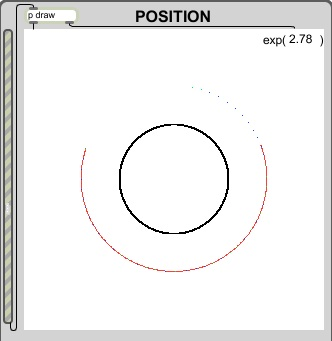
\includegraphics[width=0.4\textwidth]{circular} % Include the image placeholder.png
\caption{Circular Orbit}
\end{center}
\end{figure}

\subsection{Escape Velocity}
For the conditions $\overrightarrow{r}_0=(10,0)$ and $K=-0.1$ we calculate an initial velocity $\overrightarrow{v}_0=(0,0.14)$ will give an escape from the gravitational attraction.  We can observe in the simulation the object indeed escapes and the total energy is zero.  See the following figure.

\begin{figure}[h]
\begin{center}
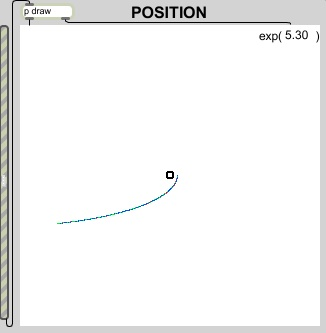
\includegraphics[width=0.4\textwidth]{escape} % Include the image placeholder.png
\caption{Escape Velocity}
\end{center}
\end{figure}

\newpage

\subsection{Elliptical Orbit}
For the conditions $\overrightarrow{r}_0=(10,0)$ and $K=-0.1$ we use an initial velocity $\overrightarrow{v}_0=(0,0.12)$ that is between the one for circular orbit and escape.  As the figure shows the resulting orbit is elliptical.

\begin{figure}[h]
\begin{center}
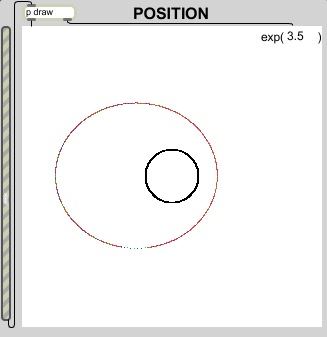
\includegraphics[width=0.4\textwidth]{elliptic} % Include the image placeholder.png
\caption{Elliptic Orbit}
\end{center}
\end{figure}
%----------------------------------------------------------------------------------------
%	SECTION 5
%----------------------------------------------------------------------------------------

\section{Discussion}



%----------------------------------------------------------------------------------------
%	SECTION 6
%----------------------------------------------------------------------------------------


%----------------------------------------------------------------------------------------
%	BIBLIOGRAPHY
%----------------------------------------------------------------------------------------

\bibliographystyle{apalike}

\bibliography{sample}

%----------------------------------------------------------------------------------------


\end{document}